Examine the data on women's national track records in Table 1.9 for marginal and multivariate normality.

For ($x_{1}$), we're looking at the Womens 100m national tract record (in seconds) for 54 countries. The simulated 0.01, 0.05, and 0.10 level critical correlation coefficient test values for a sample size of 54 are, 0.9691, 0.9784, and 0.9822, respectively. The Q-Q correlation coefficient using the raw data is 0.9836, which is larger than all three of these values, so the data would be considered normally distributed at the 0.01, 0.05, and 0.10 levels.

We don't really need to transform the data, but just to see how much better it can get, the Box-Cox power transformation max was at -4.0381, so $x_{1}^{\prime} = x_{1}^{-4.0381}$. The Q-Q correlation coefficient on the transformed data was 0.9932, so we do get a slight improvement. Below is the Q-Q plot for the raw data, which looks alright.

\begin{center}
    \begin{figure}[H]
        \centering
        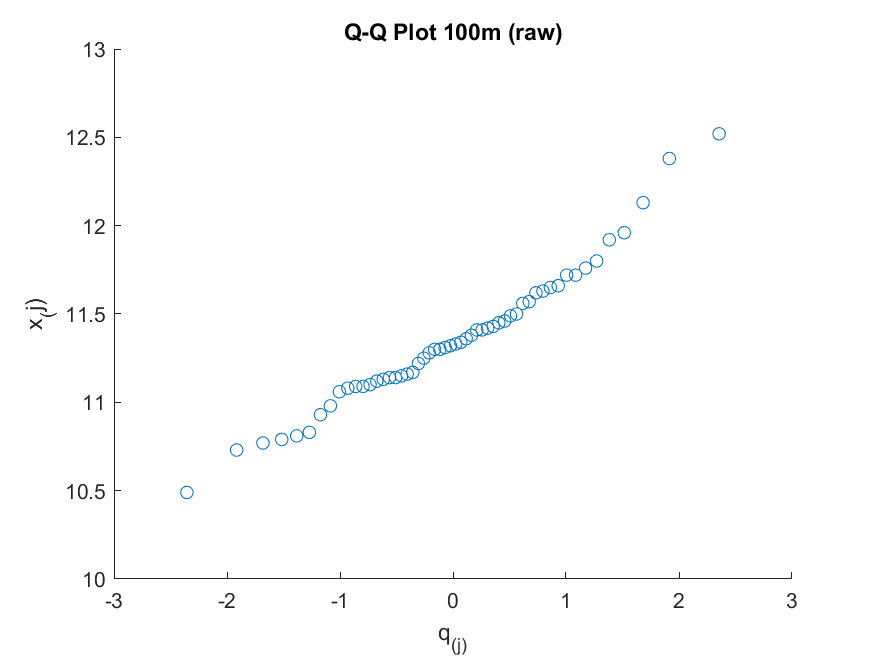
\includegraphics[scale=0.6]{./matlab/chapter-4/sol4.36.qq.1.png}
    \end{figure}
\end{center}

For ($x_{2}$), we're looking at the Womens 200m national tract record (in seconds) for 54 countries. The simulated 0.01, 0.05, and 0.10 level critical correlation coefficient test values for a sample size of 54 are, 0.9691, 0.9784, and 0.9822, respectively. The Q-Q correlation coefficient using the raw data was 0.9516, so the data would not be considered normally distributed at the 0.05 and 0.10 levels.

The transformation suggested by Box-Cox power transformation was -5.9840, but I rounded that to -6, so $x_{2}^{\prime} = x_{2}^{-6}$.
The Q-Q correlation coefficient on the transformed data was 0.9963, which is larger than all three critical values, so the data is now considered normally distributed at all three levels.
Below are the results of the power transformation and the Q-Q plots of the raw and transformed data.
The original plot shows a bit of a curve with a few large values separated out. The Q-Q plot of the transformed data was able to make the data much more linear.

\begin{center}
    \begin{figure}[H]
        \centering
        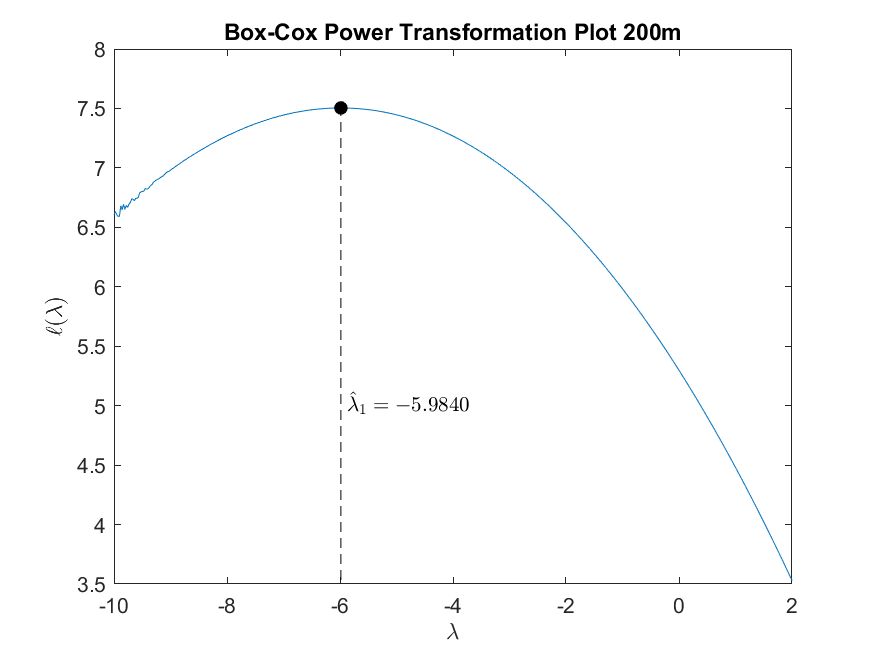
\includegraphics[scale=0.6]{./matlab/chapter-4/sol4.36.power.2.png}
    \end{figure}
\end{center}

\begin{center}
    \begin{figure}[H]
        \centering
        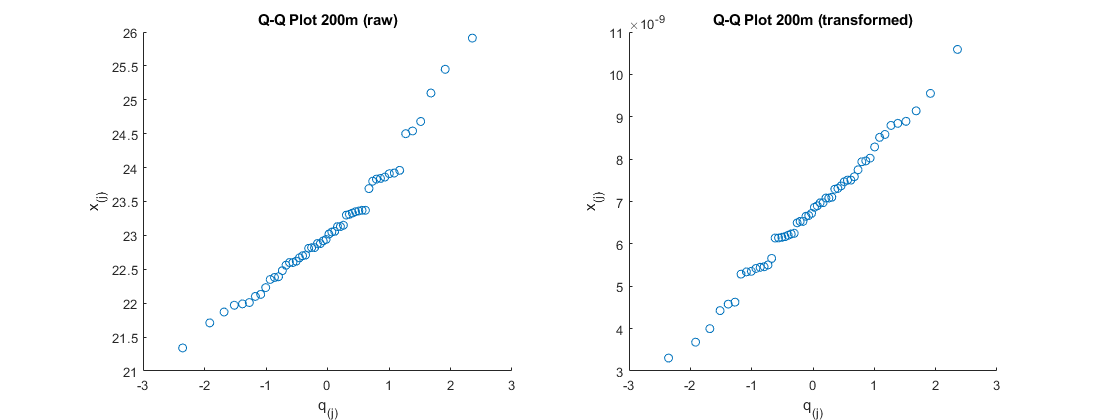
\includegraphics[scale=0.4]{./matlab/chapter-4/sol4.36.qq.2.png}
    \end{figure}
\end{center}

For ($x_{3}$), we're looking at the Womens 400m national tract record (in seconds) for 54 countries. The simulated 0.01, 0.05, and 0.10 level critical correlation coefficient test values for a sample size of 54 are, 0.9691, 0.9784, and 0.9822, respectively. The Q-Q correlation coefficient using the raw data was 0.9698, so the data would not be considered normally distributed at the 0.05 and 0.10 levels.

The transformation suggested by Box-Cox power transformation was -4.7275, but I rounded that to -4.75, so $x_{3}^{\prime} = x_{3}^{-4.75}$.
The Q-Q correlation coefficient on the transformed data was 0.9949, which is larger than all three critical values, so the data is now considered normally distributed at all three levels.
Below are the results of the power transformation and the Q-Q plots of the raw and transformed data.
The original Q-Q plot looks okay with the exception of a single outlier for the country of Cooks Island who has a 200m record of 61.65 seconds. There is no good reason to exclude this observation, so it stays. The Q-Q plot of the transformed data was able to make the data much more linear though.

\begin{center}
    \begin{figure}[H]
        \centering
        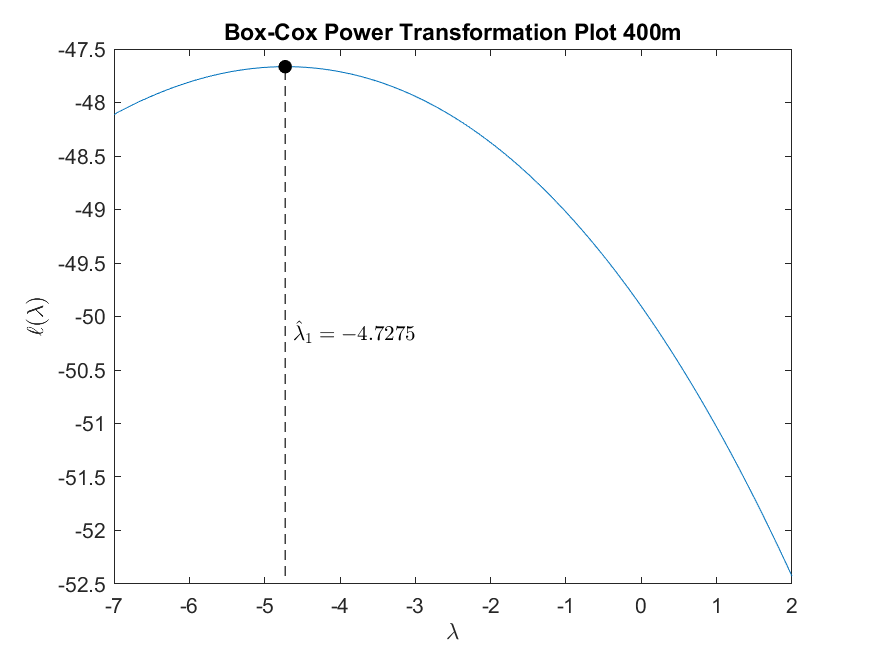
\includegraphics[scale=0.6]{./matlab/chapter-4/sol4.36.power.3.png}
    \end{figure}
\end{center}

\begin{center}
    \begin{figure}[H]
        \centering
        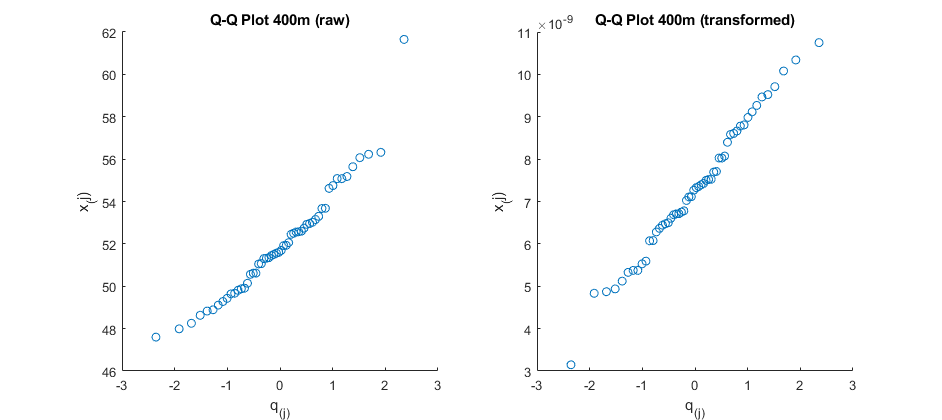
\includegraphics[scale=0.4]{./matlab/chapter-4/sol4.36.qq.3.png}
    \end{figure}
\end{center}

For ($x_{4}$), we're looking at the Womens 800m national tract record (in minutes) for 54 countries. The simulated 0.01, 0.05, and 0.10 level critical correlation coefficient test values for a sample size of 54 are, 0.9691, 0.9784, and 0.9822, respectively. The Q-Q correlation coefficient using the raw data was 0.9512, so the data would not be considered normally distributed at any of the three levels.

The transformation suggested by Box-Cox power transformation was -9.4469, but I rounded that to -9.5, so $x_{4}^{\prime} = x_{4}^{-9.5}$.
The Q-Q correlation coefficient on the transformed data was 0.9952, which is larger than all three critical values, so the data is now considered normally distributed at all three levels.
Below are the results of the power transformation and the Q-Q plots of the raw and transformed data.
The original Q-Q plot has a few large time values, where one is considered an outlier, that are reduced after the transformation. The Q-Q plot of the transformed data looks much better.

\begin{center}
    \begin{figure}[H]
        \centering
        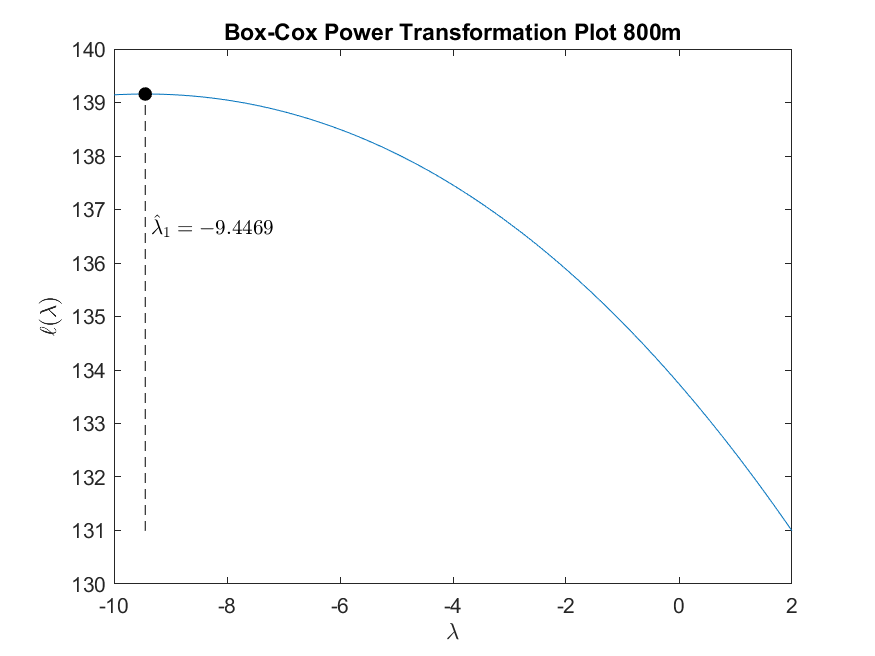
\includegraphics[scale=0.6]{./matlab/chapter-4/sol4.36.power.4.png}
    \end{figure}
\end{center}

\begin{center}
    \begin{figure}[H]
        \centering
        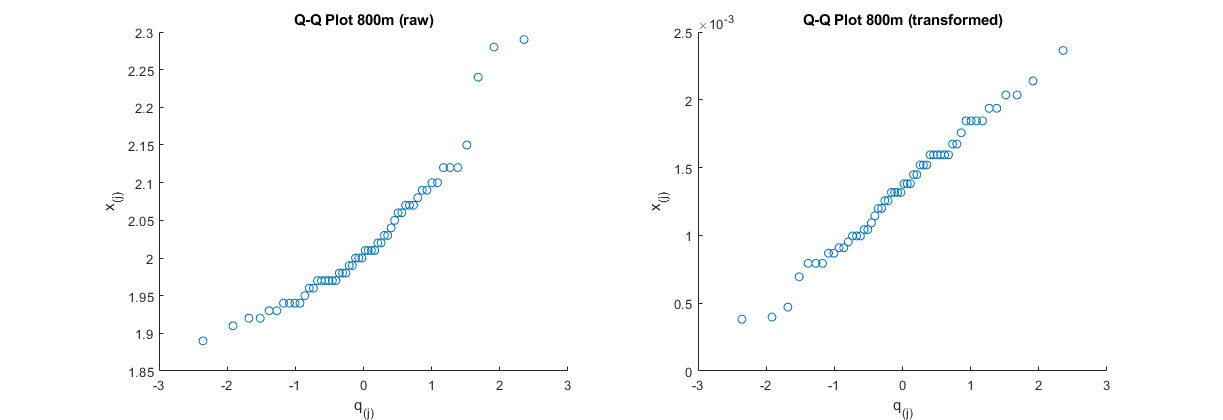
\includegraphics[scale=0.4]{./matlab/chapter-4/sol4.36.qq.4.png}
    \end{figure}
\end{center}

For ($x_{5}$), we're looking at the Womens 1500m national tract record (in minutes) for 54 countries. The simulated 0.01, 0.05, and 0.10 level critical correlation coefficient test values for a sample size of 54 are, 0.9691, 0.9784, and 0.9822, respectively. The Q-Q correlation coefficient using the raw data was 0.91, so the data would not be considered normally distributed at any of the three levels.

The transformation suggested by Box-Cox power transformation was -8.1002, but I rounded that to -8, so $x_{5}^{\prime} = x_{5}^{-8}$.
The Q-Q correlation coefficient on the transformed data was 0.9921, which is larger than all three critical values, so the data is now considered normally distributed at all three levels.
Below are the results of the power transformation and the Q-Q plots of the raw and transformed data.
The original Q-Q plot has an outlier for the country of Samoa (5.42 min), that's reduced after the transformation. The Q-Q plot of the transformed data looks much better.

\begin{center}
    \begin{figure}[H]
        \centering
        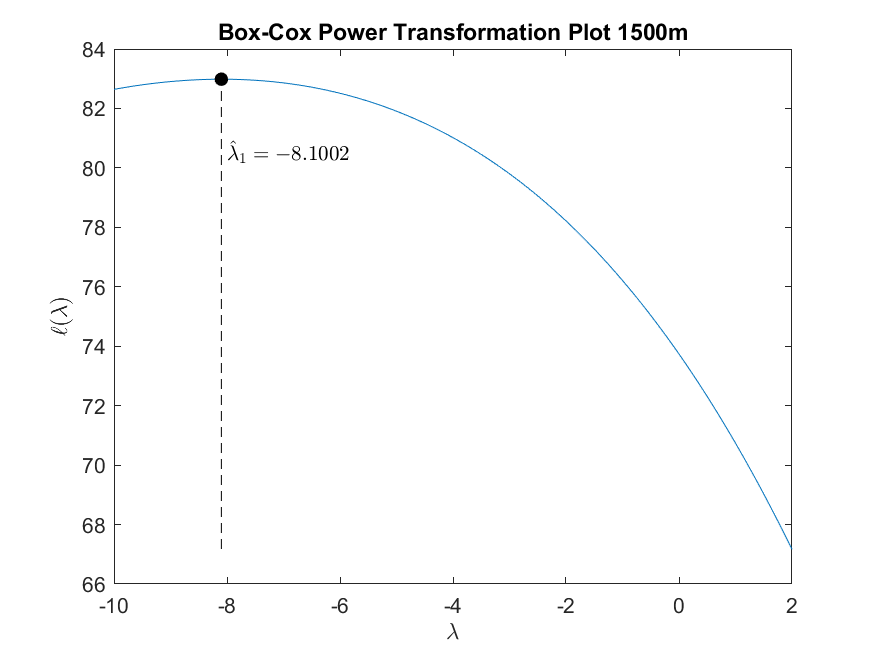
\includegraphics[scale=0.6]{./matlab/chapter-4/sol4.36.power.5.png}
    \end{figure}
\end{center}

\begin{center}
    \begin{figure}[H]
        \centering
        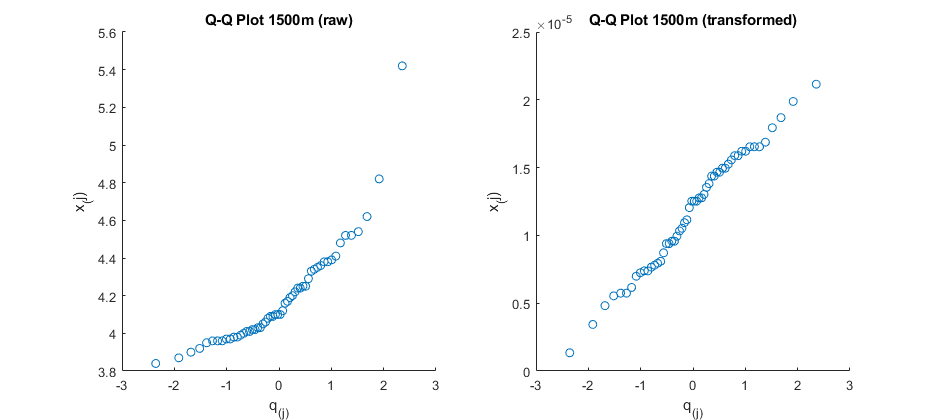
\includegraphics[scale=0.4]{./matlab/chapter-4/sol4.36.qq.5.png}
    \end{figure}
\end{center}

For ($x_{6}$), we're looking at the Womens 3000m national tract record (in minutes) for 54 countries. The simulated 0.01, 0.05, and 0.10 level critical correlation coefficient test values for a sample size of 54 are, 0.9691, 0.9784, and 0.9822, respectively. The Q-Q correlation coefficient using the raw data was 0.8677, so the data would not be considered normally distributed at any of the three levels.

The transformation suggested by Box-Cox power transformation was -7.1623, but I rounded that to -7.2, so $x_{6}^{\prime} = x_{6}^{-7.2}$.
The Q-Q correlation coefficient on the transformed data was 0.9897, which is larger than all three critical values, so the data is now considered normally distributed at all three levels.
Below are the results of the power transformation and the Q-Q plots of the raw and transformed data.
The original Q-Q plot has an outlier for the country of Samoa (13.12 min), that's reduced after the transformation. The Q-Q plot of the transformed data looks somewhat better.

\begin{center}
    \begin{figure}[H]
        \centering
        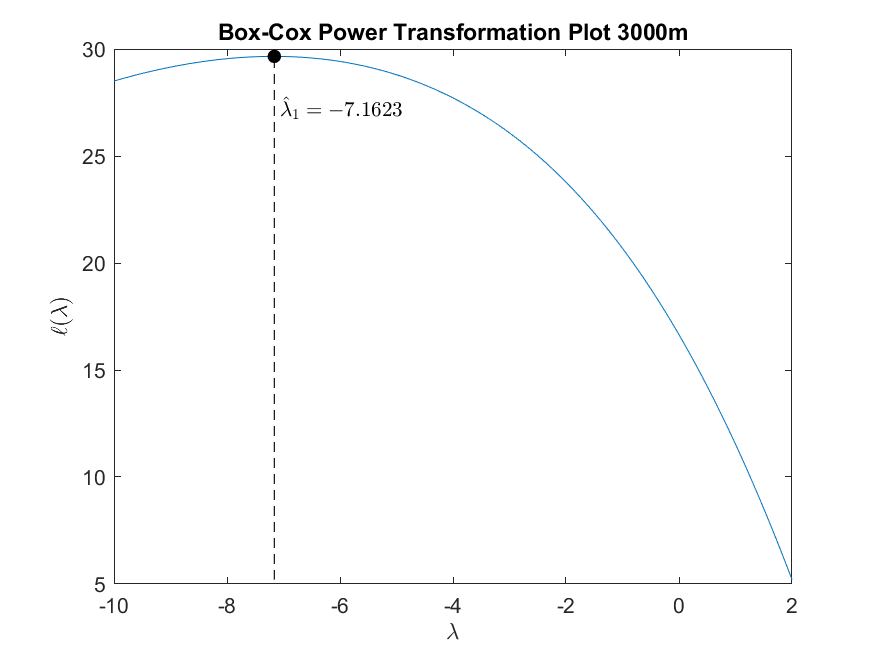
\includegraphics[scale=0.6]{./matlab/chapter-4/sol4.36.power.6.png}
    \end{figure}
\end{center}

\begin{center}
    \begin{figure}[H]
        \centering
        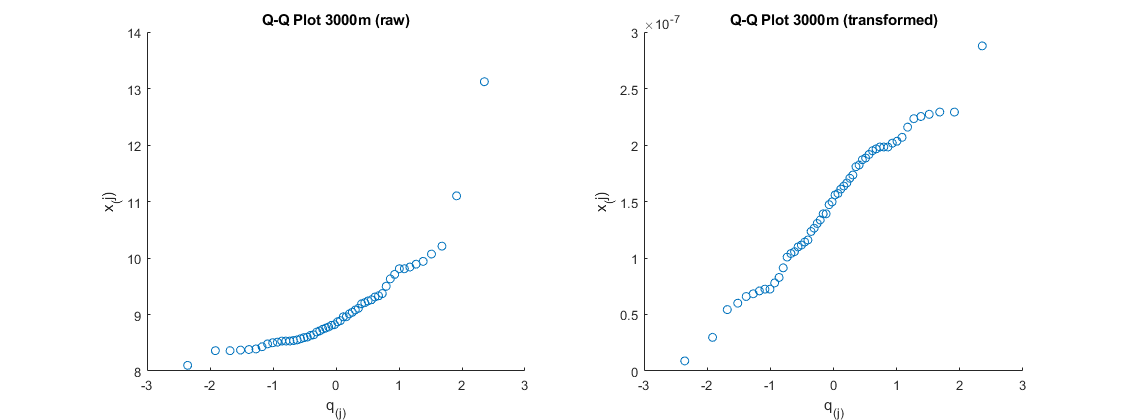
\includegraphics[scale=0.4]{./matlab/chapter-4/sol4.36.qq.6.png}
    \end{figure}
\end{center}

For ($x_{7}$), we're looking at the Womens marathon national tract record (in minutes) for 54 countries. The simulated 0.01, 0.05, and 0.10 level critical correlation coefficient test values for a sample size of 54 are, 0.9691, 0.9784, and 0.9822, respectively. The Q-Q correlation coefficient using the raw data was 0.8606, so the data would not be considered normally distributed at any of the three levels.

The transformation suggested by Box-Cox power transformation was -6.9098, but I rounded that to -7, so $x_{7}^{\prime} = x_{7}^{-7}$.
The Q-Q correlation coefficient on the transformed data was 0.9935, which is larger than all three critical values, so the data is now considered normally distributed at all three levels.
Below are the results of the power transformation and the Q-Q plots of the raw and transformed data.
The original Q-Q plot has two outliers. One for Papua New Guinea (221.14 min), and the other for Cook Islands (212.33 min). Both are reduced after the transformation. The Q-Q plot of the transformed data looks somewhat better.

\begin{center}
    \begin{figure}[H]
        \centering
        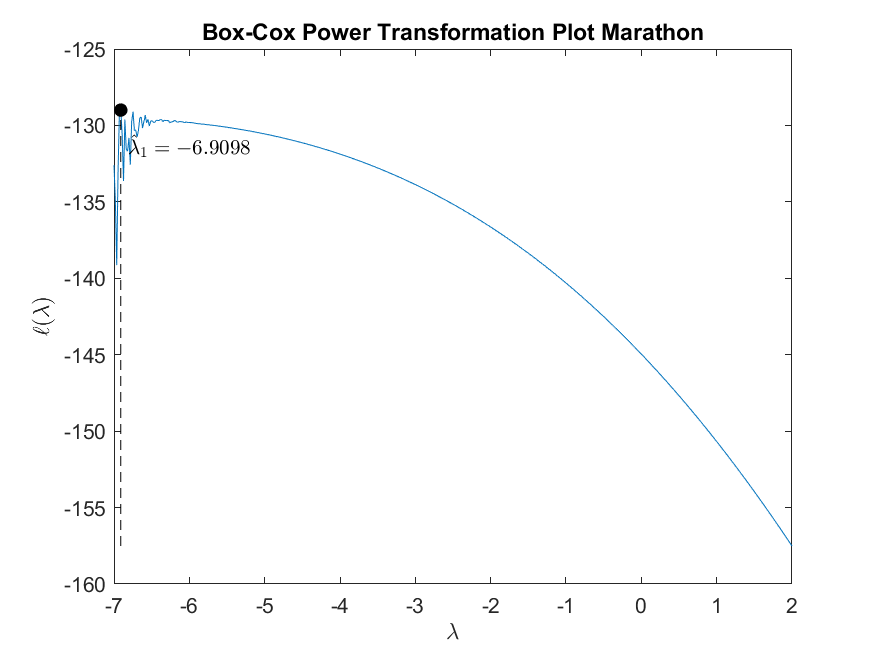
\includegraphics[scale=0.6]{./matlab/chapter-4/sol4.36.power.7.png}
    \end{figure}
\end{center}

\begin{center}
    \begin{figure}[H]
        \centering
        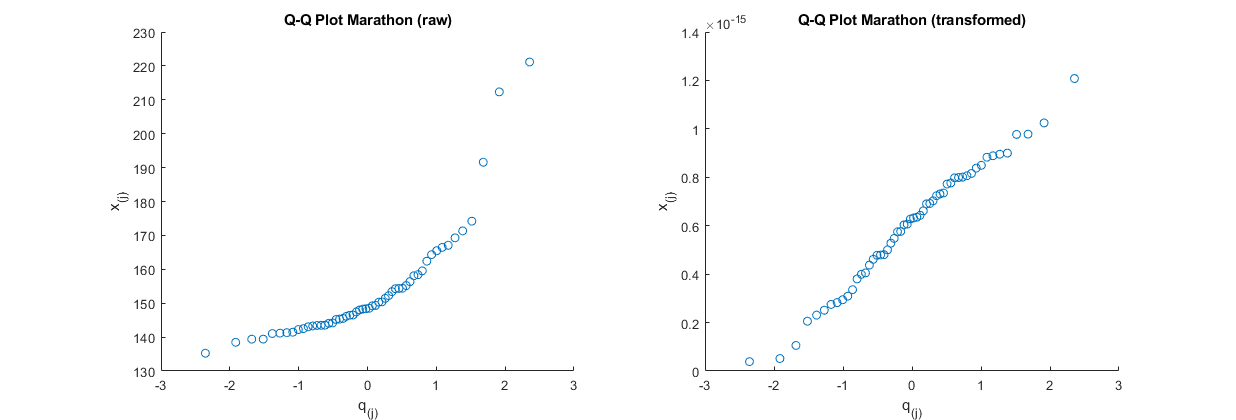
\includegraphics[scale=0.4]{./matlab/chapter-4/sol4.36.qq.7.png}
    \end{figure}
\end{center}

Computing the statistical distance based on our 7 covariates and creating a Chi-Squared plot (below). The raw data on the left  shows 5 observations with statistical distances larger than most of the data. The transformed data on the right does show some improvement, but there are 3 observation with larger statistical distances than the others They are, North Korea (19.5334), Czech Republic (18.7619), and Mexico (18.0769). Without them the overall data would appear much more normal, but assuming these are not measurement errors, these observations will have to stay.

\begin{center}
    \begin{figure}[H]
        \centering
        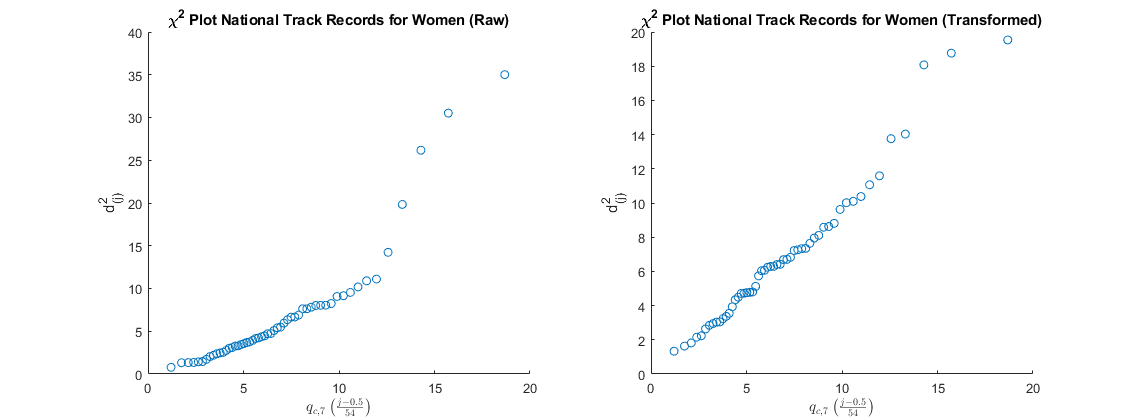
\includegraphics[scale=0.4]{./matlab/chapter-4/sol4.36.chi2.png}
    \end{figure}
\end{center}


